\section{Complex exponentials review}
\begin{enumerate}
\item $e^{xi}$ is a point on the unit circle.
\item $e^{2\pi i} = 1$ i.e. one full rotation.
\item $r(t) = e^{2\pi i t}$ is a function describing a point moving on the unit circle. If $t$ is in seconds then
  this point will perform one cycle per second (1 Hz).
\item $r(t) = e^{2\pi i f t}$ is a point rotating at a frequency of $f$ Hz. (E.g. if $f = 2$ then it will get to
  the same position in half the time.)
\end{enumerate}

\section{Fourier transform}

Let $g(t)$ be a non-negative 1D continuous time series. Consider the function
\begin{align*}
  g(t)e^{-2\pi i f t}.
\end{align*}
This represents ``winding'' the time series around the unit circle (the negative sign means we are winding
clockwise).

\begin{mdframed}
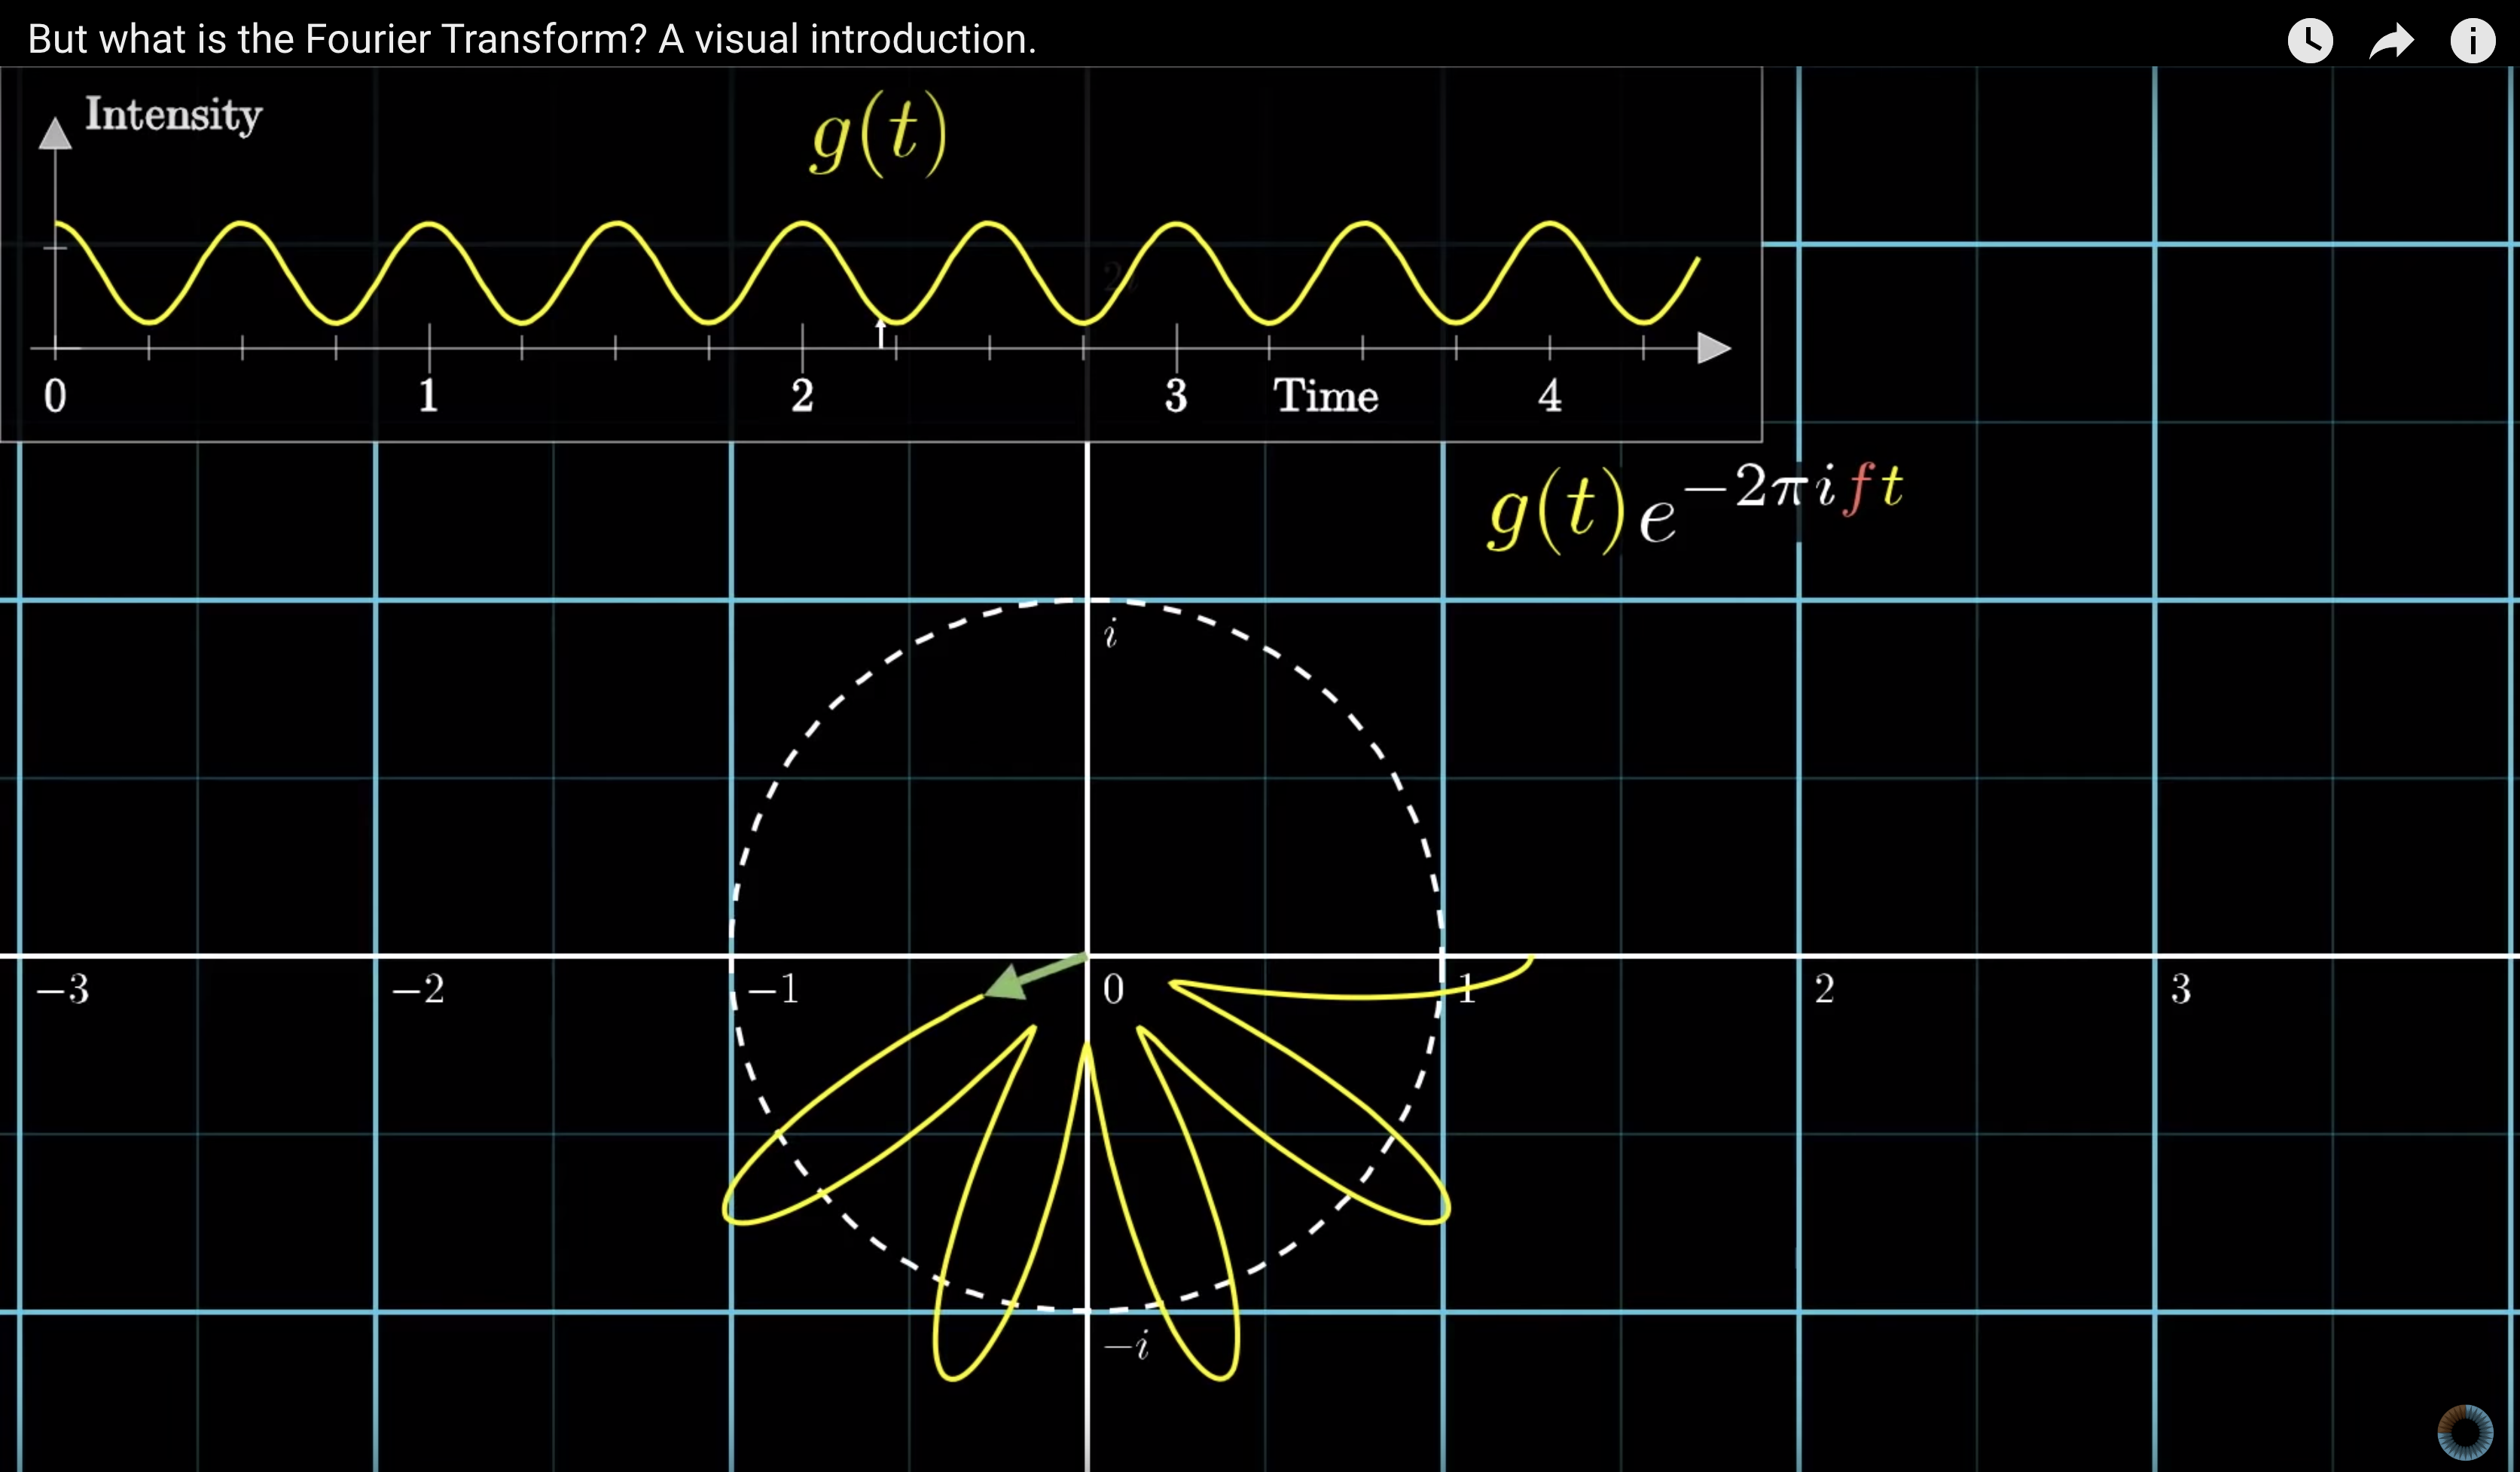
\includegraphics[width=400pt]{img/fourier--complex-exponentials-review--fourier-transform-75f4.png}
\end{mdframed}

$f$ controls the winding frequency: if $f = 1$ then the function winds around once in $2\pi$ seconds;
if $f = 2$ then the function winds around once in $\pi$ seconds.

Note that there are two frequency concepts here:
\begin{enumerate}
\item The time series $g(t)$ is composed of some mixture of sinusoids, each with a certain frequency.
\item The winding frequency $f$.

  The Fourier transform basically involves computing a ``centre of mass'' of the wound-up time series, for a
  range of $f$ values.

For most $f$ values, the centre of mass will be close to the origin.
\begin{mdframed}
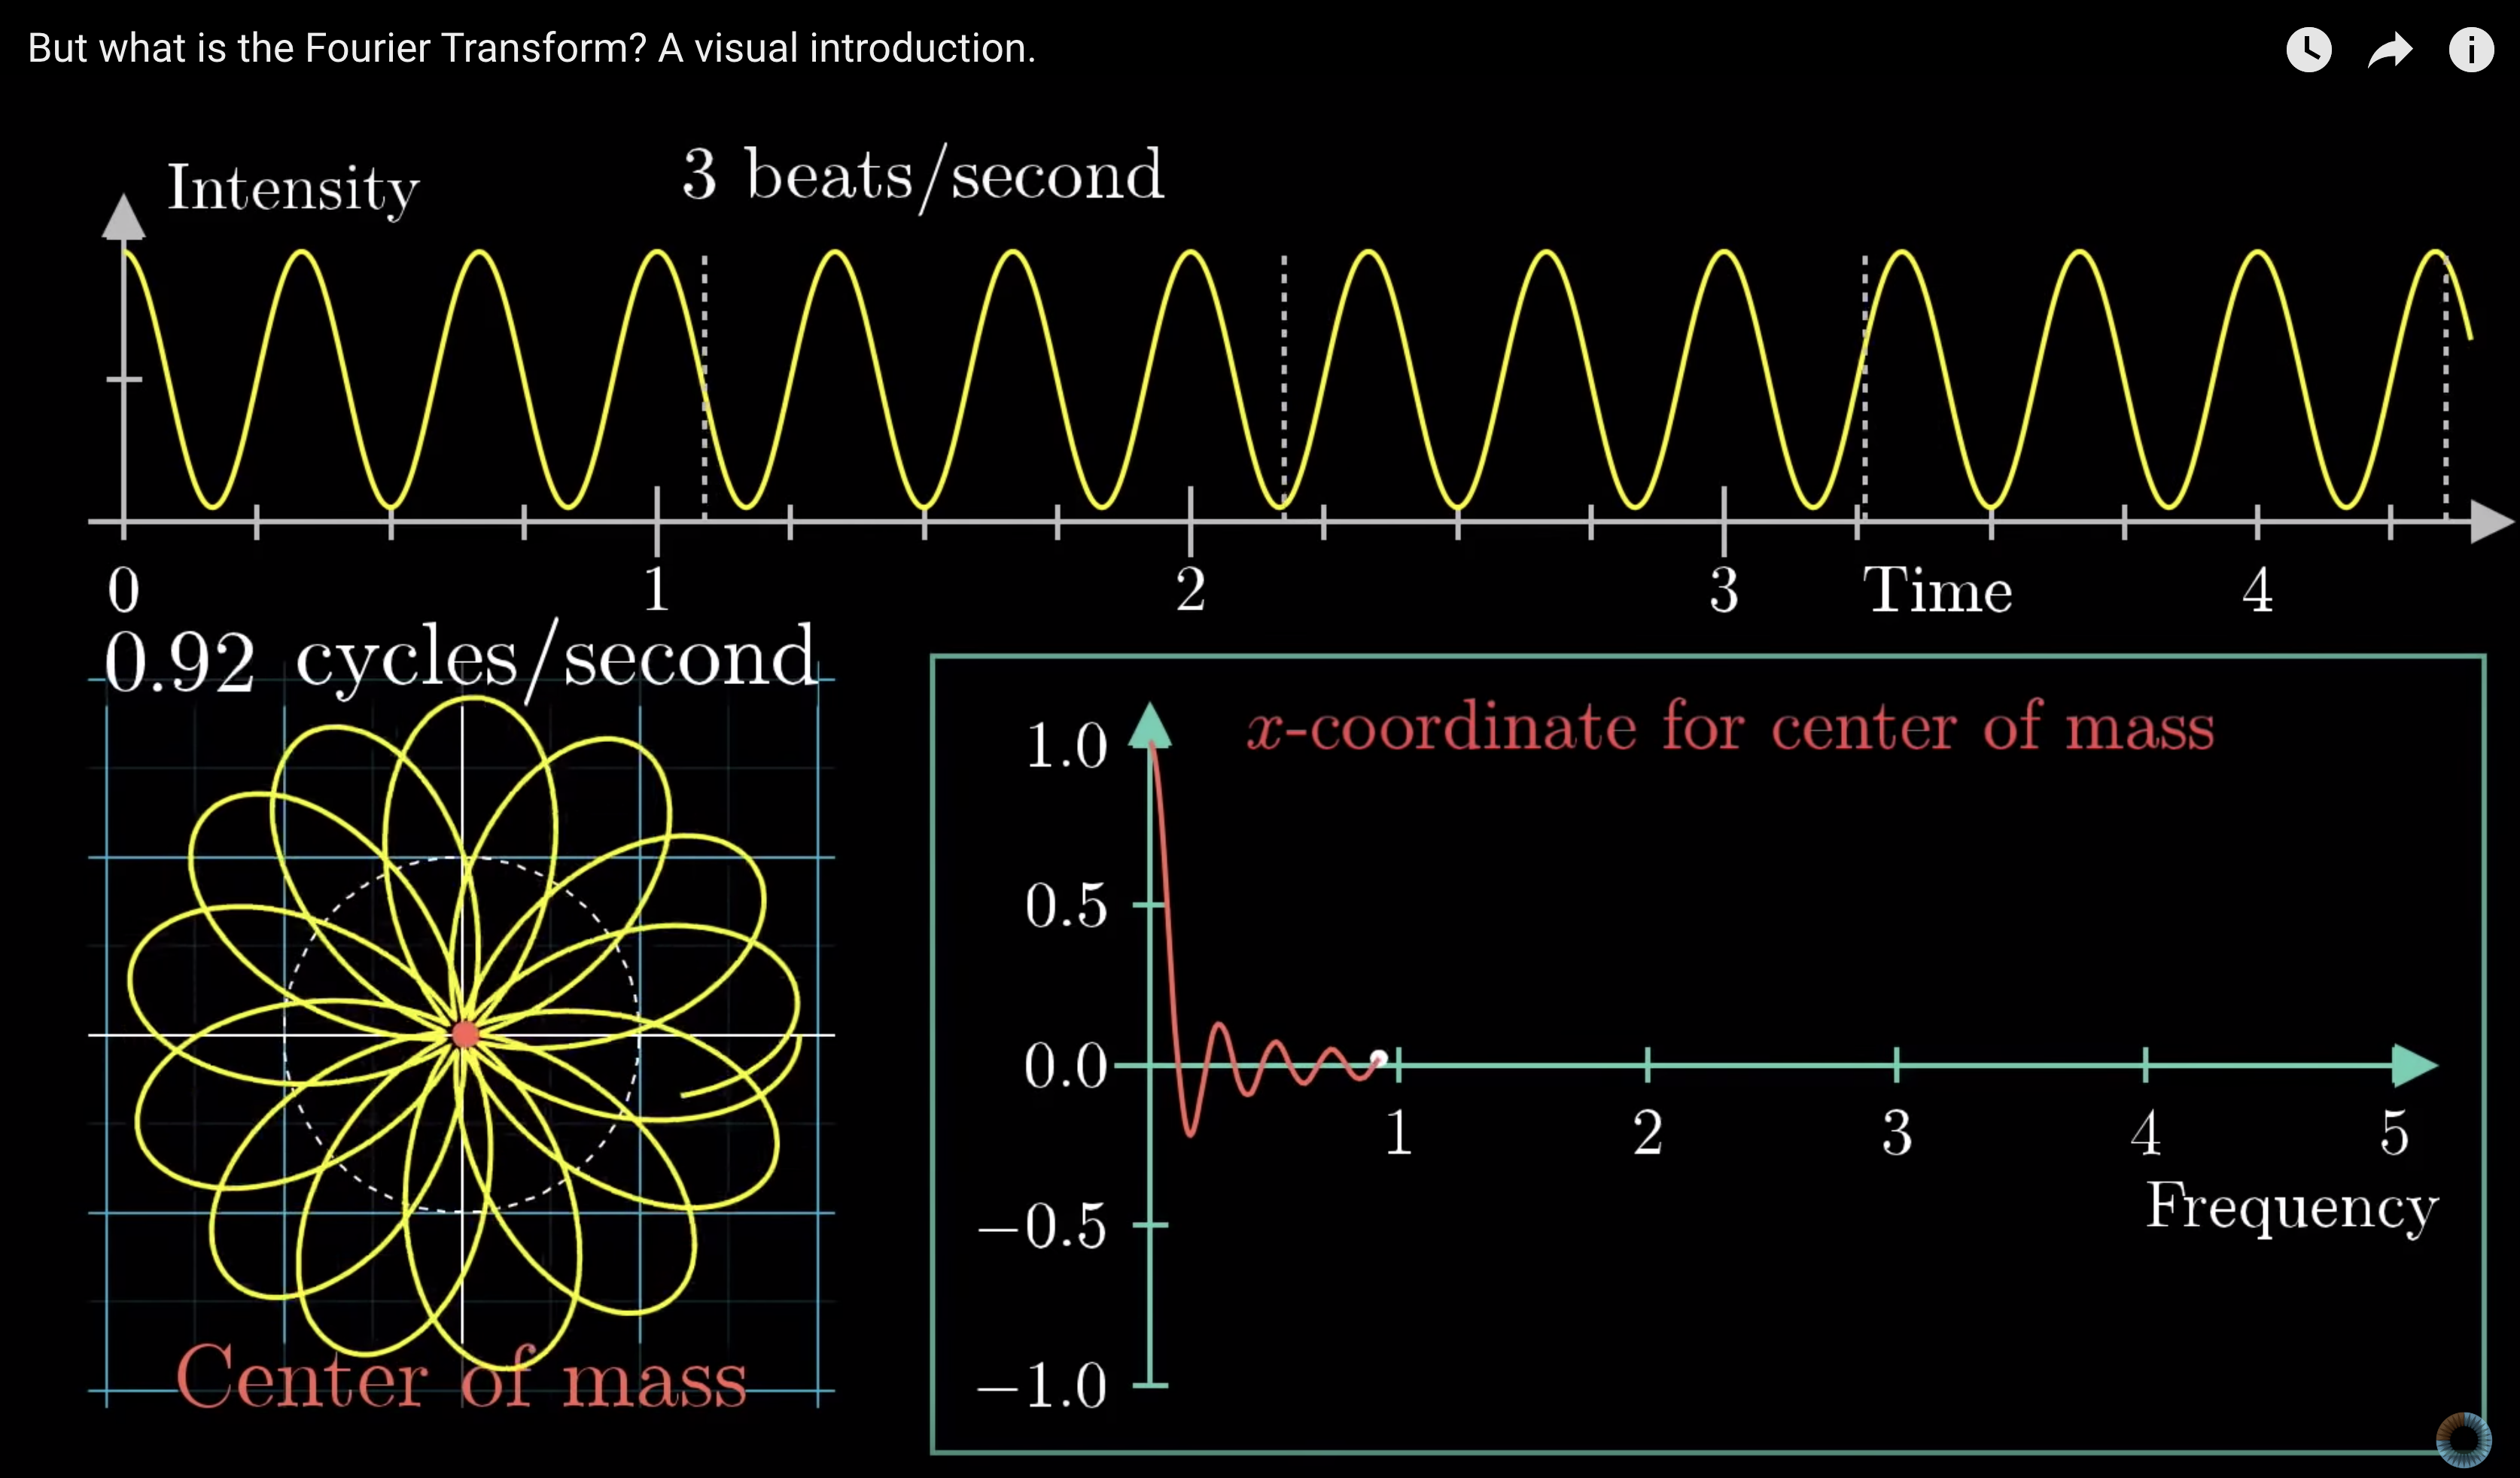
\includegraphics[width=400pt]{img/fourier--complex-exponentials-review--fourier-transform-eca1.png}
\end{mdframed}

But occasionally one will hit an $f$ value that ``resonates'' with one of the frequency components of the time
series: when this happens, the peaks of $g(t)$ will coincide, on the same side of the unit circle, and the
centre of mass will thus be far from the origin.
\begin{mdframed}
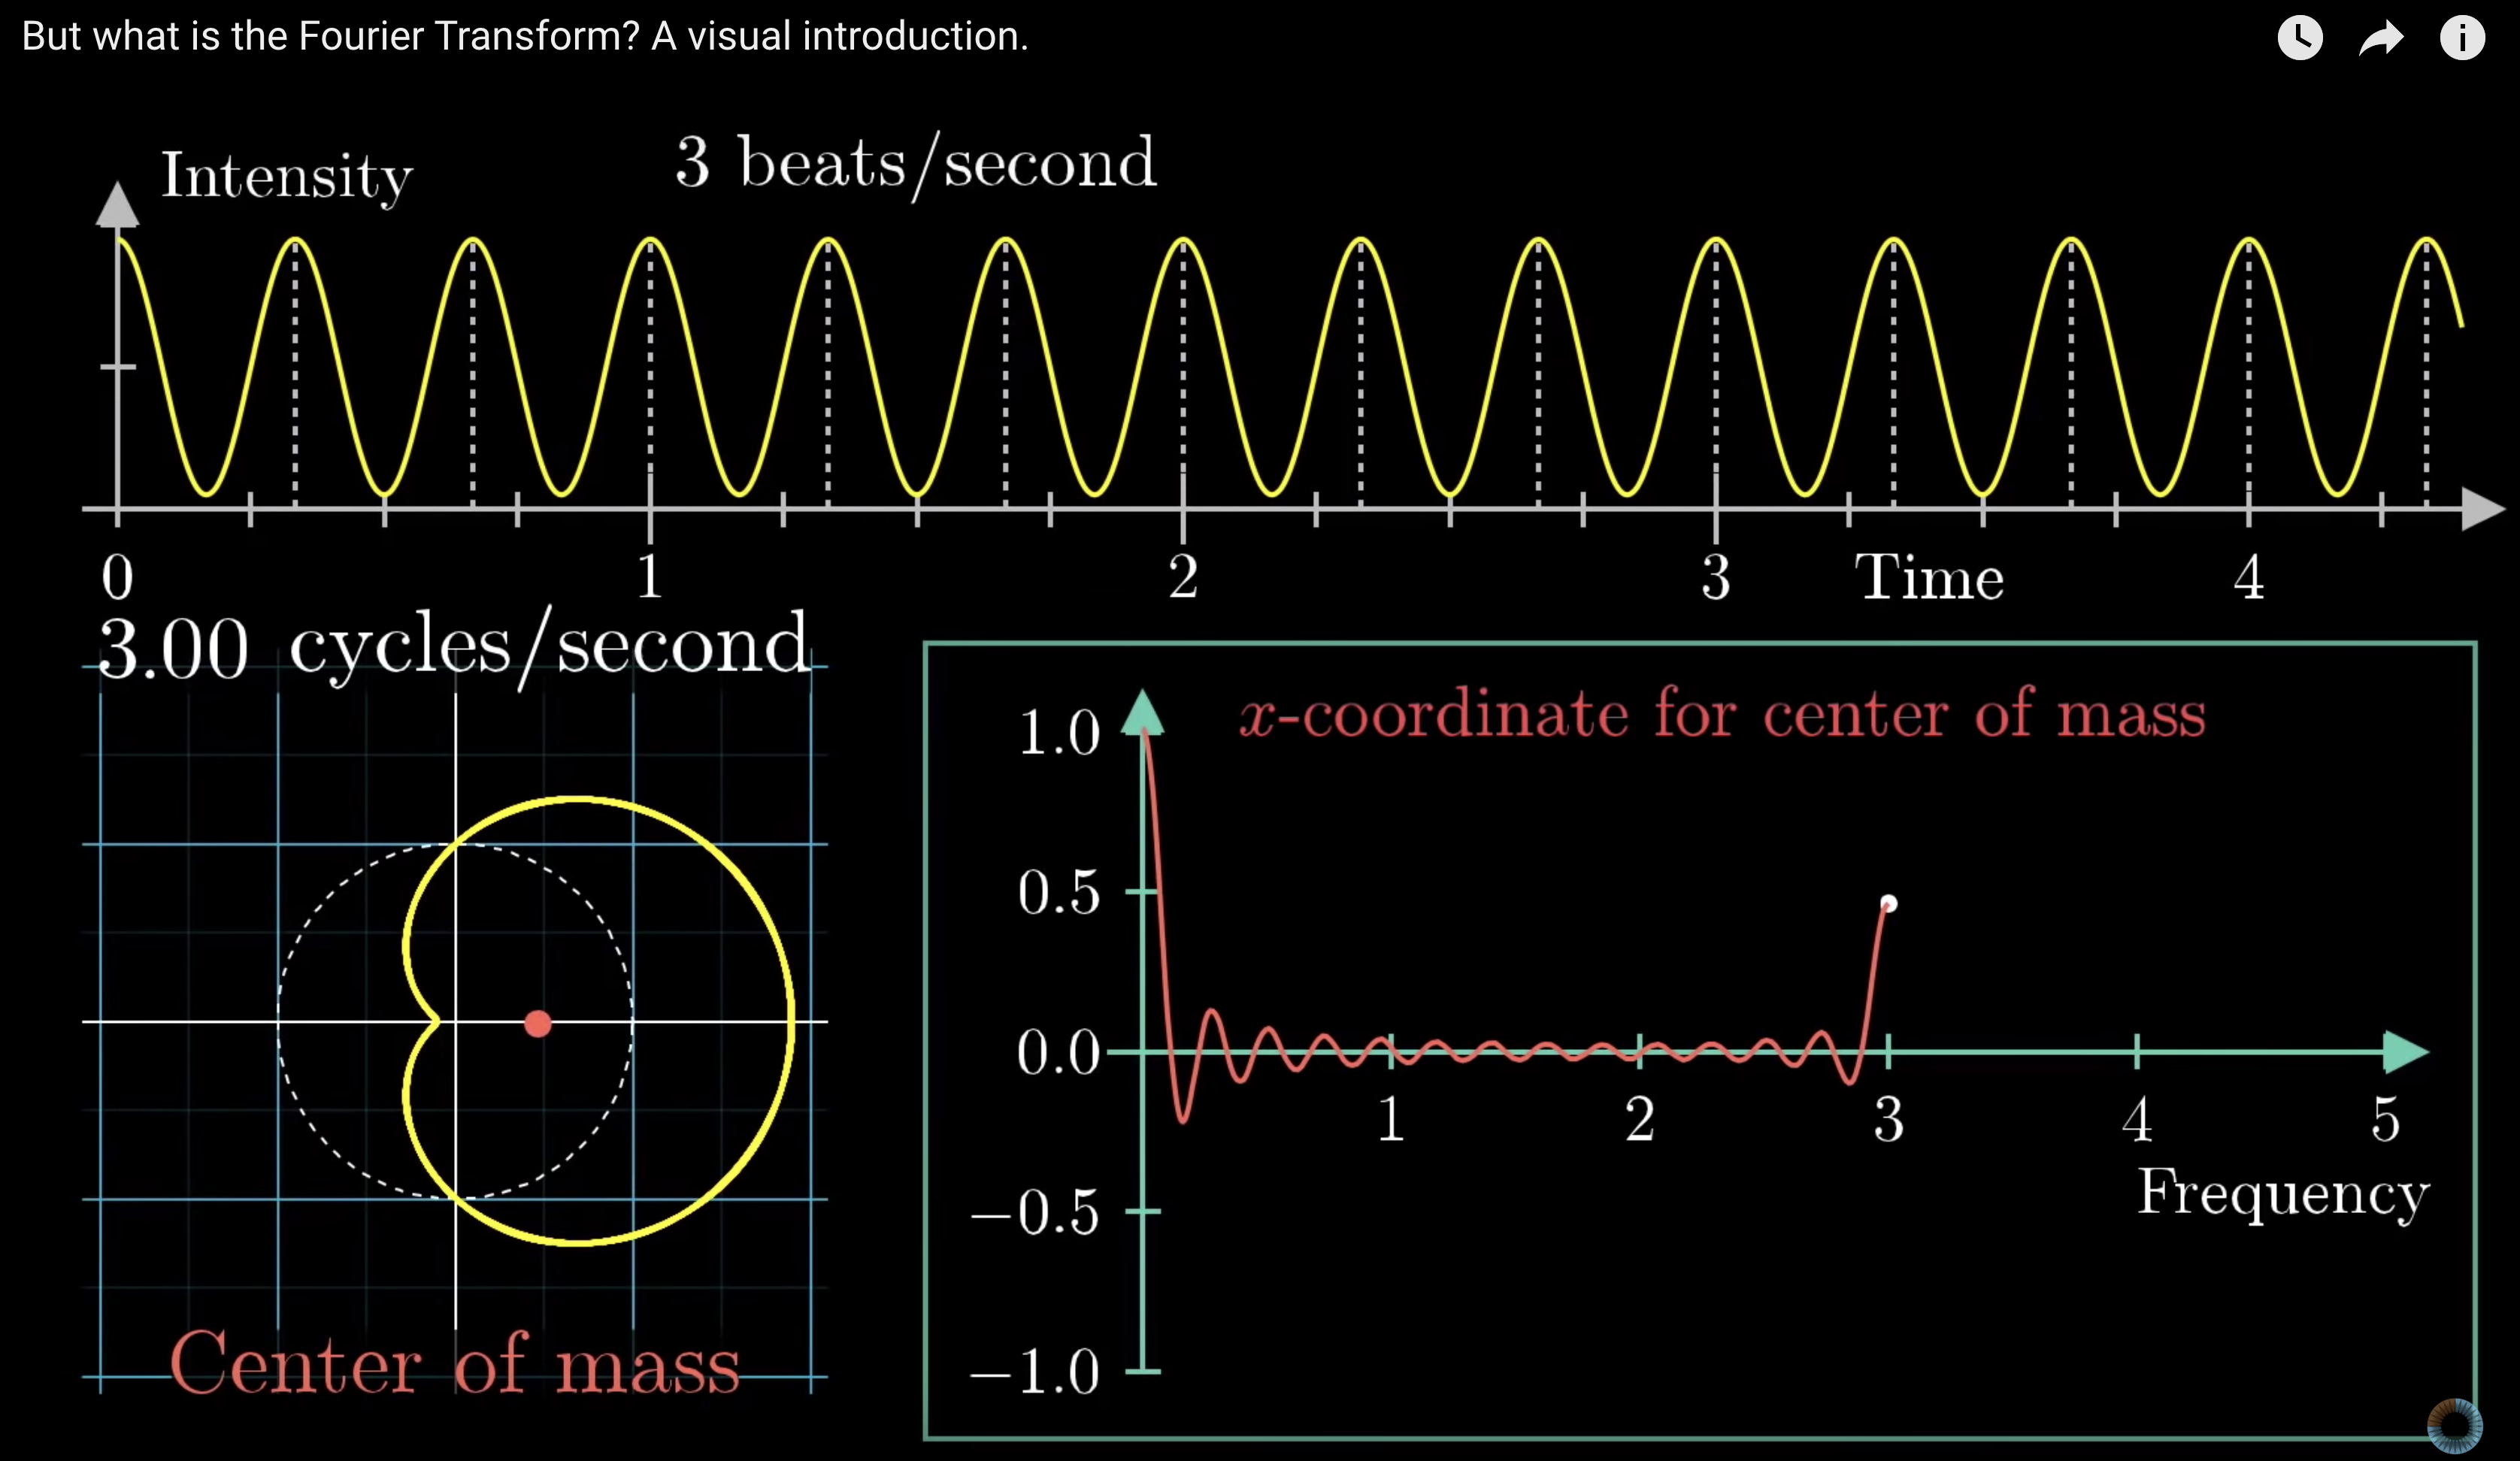
\includegraphics[width=400pt]{img/fourier--complex-exponentials-review--fourier-transform-f265.png}
\end{mdframed}
\end{enumerate}
The ``centre of mass'' of the wound-up curve is
\begin{align*}
  \frac{1}{t_2 - t_1} \int_{t_1}^{t_2} g(t)e^{-2\pi i f t} \dt.
\end{align*}
However, the Fourier transform is defined without the division, and over all time:
\begin{align*}
  \hat{g}(f) := \int_{-\infty}^{\infty} g(t)e^{-2\pi i f t} \dt.
\end{align*}
Note that $\hat{g}(f)$ is complex-valued (the centre of mass is a point in the complex plane). Often one might
just look at its real component (why not look at the modulus?).

Thye fact that one does not divide by the sampled time duration means that if a signal of frequency $f^*$
persists for a long time, then $\hat{g}(f^*)$ will be large: i.e. the Fourier transform emphasizes frequencies
that are present for more time.

\footnote{\url{https://www.youtube.com/watch?v=spUNpyF58BY}}
